\documentclass[11pt]{article}
\usepackage{amsmath,amssymb,graphicx}
\usepackage[letterpaper ,left=2cm,top=2.25cm,bottom=2.25cm,right=2.5cm,nohead,nofoot]{geometry}
\usepackage{color}
\usepackage{bm}
\usepackage{bbold}
\renewcommand{\vec}[1]{\mathbf{#1}}
\DeclareMathOperator{\sgn}{sgn}
\pagestyle{empty}
\usepackage[T1]{fontenc}
%\usepackage{times}
\IfFileExists{newtxtext.sty}
   {\usepackage{newtxtext,newtxmath}}
   {\IfFileExists{stix.sty}
      {\usepackage{stix}}
      {\IfFileExists{mathptmx.sty}
      {\usepackage{mathptmx}}{} } }
\usepackage[scaled]{beramono}
\begin{document}

\begin{center}
{\large\bf Physics 540: Class 17}\\
{\small Wednesday, June 23, 2021}
\end{center}

The shape of a string suspended from two fixed points is called a \emph{catenary} and has the well-known form
\[ y(x) = a[\cosh((x-x_0)/a)-1] + y_0.\] 
The parameters $x_0$ and $y_0$ are translations, and $a = \rho g$ is a product of the line tension of the string
and the local gravitational acceleration. We're going to use measurements to fit these three unknowns (of which
only $a$ is physically meaningful).

To start, compile and run the \verb!catenary! program:
{\small\begin{verbatim}
$ make catenary
g++ -c catenary.cpp -O2 -ansi -pedantic -Wall
g++ -c catenary_openGL.cpp -O2 -ansi -pedantic -Wall
g++ -o catenary catenary.o catenary_openGL.o  -framework OpenGL -framework GLUT -lobjc
$ ./catenary
\end{verbatim}}
Maximize the window so that it covers most of your screen. Then, hang a piece of string from the two sides of your monitor. 
Using your mouse, carefully trace the path of the string using 20 to 50 clicks. Press `n' to start a new set of measurements.
Repeat this at least ten times. Press `q' to quit the program. You should find that your measurements are stored
in a file named \verb!string.dat!:
{\small\begin{verbatim}
$ more string.dat
$ gnuplot
> plot "string.dat"
> plot "string.dat" index 0
> plot "string.dat" index 1
> plot "string.dat" index 2
> quit
\end{verbatim}}

The non-negative quantity
 \[ \chi^2 = \sum_{i=1}^N (y-y_i)^2 =  \sum_{i=1}^N (\Delta y_i)^2 = \sum_{i=1}^N \biggl[a \cosh\biggl(\frac{x_i-x_0}{a}\biggr)-a + y_0-y_i\biggr]^2 
 \] 
 measures the deviation of the measured data from the predicted curve for a particular set of parameters $(x_0,y_0,a)$.
 The best possible fit corresponds to the smallest value of $\chi^2$. 
 The derivatives of $\chi^2$ along each of the parameter directions are summarized below.  
 \begin{align*}
 \frac{\partial\chi^2}{\partial x_0} &= -\sum_{i=1}^N \Delta y_i \sinh\biggl(\frac{x_i-x_0}{a}\biggr)\\
 \frac{\partial\chi^2}{ \partial y_0} &= \sum_{i=1}^N \Delta y_i\\
 \frac{\partial \chi^2}{\partial a} &= \sum_{i=1}^N \Delta y_i \biggl[ \cosh\biggl(\frac{x_i-x_0}{a}\biggr) - 1 - \biggl(\frac{x_i-x_0}{a}\biggr) \sinh\biggl(\frac{x_i-x_0}{a}\biggr) \biggr]
 \end{align*}
We can think of the three parameters as constituting a vector 
$\mathbf{v} = (v_1, v_2, v_3) \equiv (x_0, y_0, a)$ whose local downhill direction is given by the gradient
$-\partial \chi^2/\partial v_i$. 

The program \verb!string_fit! is designed to read in your measurements from \verb!string.dat! and fit a catenary
curve to it. A bootstrapping technique is used in which the fit is performed repeatedly on a random sample
of the data. The mean and variance of the parameters then provide a best fit value and a statistical uncertainty.

In the file \verb!string_fit.cpp!, write routines \verb!steepest_descent!
and \verb!statistics! that (i) compute the best-fit value
of $\mathbf{v}$ using steepest descent and (ii) compute the mean and variance of a list of bootstrap samples.
A completed program will give you results something like the following and a nice graph.
{\small\begin{verbatim}
$ ./string_fit
Processing...
iteration 1
iteration 2
iteration 3
.
.
iteration 95
iteration 96
iteration 97
iteration 98
iteration 99
iteration 100
  x0 = -0.01583404978 +/- 0.00045
  y0 = -0.3950524019 +/- 0.0032
   a = 1.044980718 +/- 0.003
$ gnuplot -persist view.gp
\end{verbatim}}
\begin{center}
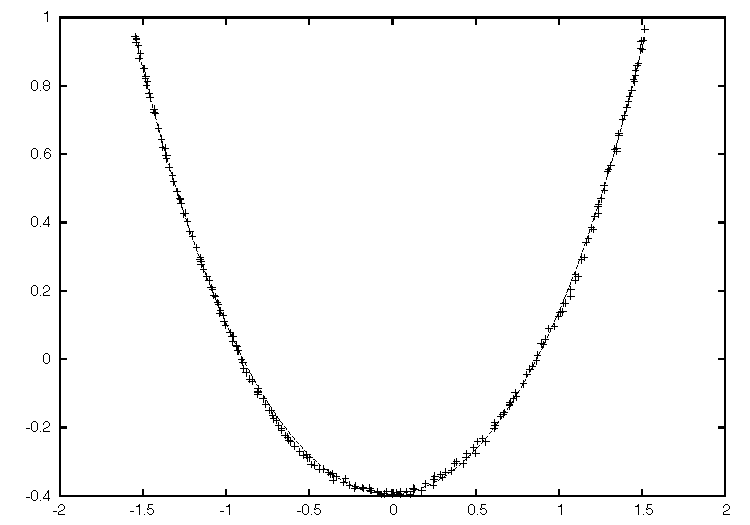
\includegraphics{catenary.pdf}
\end{center}

\end{document}